\section{Explaining a DNN with Concept Localization and ILP}
% One approach to explainability is to find an approximate, more
% interpretable, logical representation of the internal processing of a
% given DNN.
% Such representations are built from propositional (boolean or fuzzy)
% logic, \idest \texttt{if-then-else}-blocks, together with domain
% specific predicates like \ilprule{isa(\dots)} or
% \ilprule{contains}.
% The \emph{expressive power} \cite{tickle_truth_1998} of a method
% refers to the complexity of facts that can be covered. This is
% limited by the logic used.
% Especially, the better the set of predicates covers relations the DNN
% is capable to use, the better the DNN can be approximated without loss
% of interpretability.
% For example, spatial relations like \ilprule{top\_of} or
% \ilprule{right\_of}, and negations should be covered:
% They may be used by a fully connected unit of a DNN or---within the
% range of its receptive field---by a convolutional filter.

When building explanations for a DNN via approximate rule sets,
the underlying logic and predicates of the rules should reflect the
capabilities of the model.
For example, spatial relations like \ilprule{top\_of} or
\ilprule{right\_of} should be covered, as \forexample dense
layers of a DNN are capable of encoding these.
% 
Spatial relations cannot be represented by current visualization
methods for explainable AI, which only feature predicates of the form
\ilprule{contains(Example, Part)} and \ilprule{at\_position(Part, xy)}.
% The same holds for traditional rule extraction
% techniques \cite{hailesilassie_rule_2016}.
Rule-based methods like ILP are able to incorporate richer
predicates into the output. However, their input must be symbolic background
knowledge about the training and inference samples which
is formulated using these predicates \emph{explicitly}.
% For example, given all of
% \begin{quote}
%   \ilprule{(eye in image,
%   eye closed,
%   mouth in image,
%   mouth open)}
% \end{quote}
% this may be evaluated to \enquote{person asleep} given the rule
% \begin{quote}
%   \ilprule{(eye in image, eye closed)
%   $\rightarrow$ person asleep}.
% \end{quote}
For computer vision tasks with pixel-level input, this
encoding of the background knowledge about samples is not available.
% 
To remedy this, we propose to use existing concept mining techniques
for extraction of the required background knowledge:
\begin{enumerate}
\item Associate pre-defined visual semantic concepts with
  intermediate output of the DNN.
  Concepts can be local, like parts and textures, or image-level.
\item Automatically infer the background knowledge about a sample
  \ilprule{Ex} given the additional concept output, which defines
  predicates
  \ilprule{isa(C, concept)}, and
  \ilprule{isa(Ex, C)} (image-level) or
  \ilprule{contains(Ex, C)} with \ilprule{at\_position(C, xy)}.
  From this, spatial relations and negations can be extracted.
\item Given background knowledge for a set of training samples,
  apply an inductive logic programming approach to learn an
  expressive set of rules for the DNN.
\end{enumerate}

The approach presented in this paper differs from the previous work
outlined in \cite{rabold2019enriching} by the following main aspects:

\begin{itemize}
\item We will find a global verbal explanation for a black-box
  decision in contrast to a local explanation.
\item We directly make use of information stored in the building
  blocks of the DNN instead of relying on the linear surrogate
  model generated by LIME.
\end{itemize}

\subsection{Enrich DNN Output via Concept Embedding Analysis}
We directly built upon the concept detection approach
from \cite{fong_net2vec_2018,schwalbe_concept_2020}, suggesting some
further improvements.
% upscaling
% The method in \cite{schwalbe_concept_2020} downscales and binarizes
% the ground truth masks to not overly penalize the low resolution of
% activation maps compared to the input image. However, this may lead to
% a loss of ground truth information if the resolution is too low: In
% case of smaller concepts like a nose the segmentation may get lost
% completely.
Net2Vec bilinearly upscaled the predicted masks before
applying the sigmoid for logistic regression.
This overrates the contribution to the loss by pixels at
the edges from positive to negative predicted pixels. We instead
apply upscaling after applying the sigmoid.
% 
%%% loss
Instead of the suggested IoU penalty from
\cite{schwalbe_concept_2020}, we propose a more stable
Dice loss to fit the overlap objective, supported by a small summand
of the balanced binary cross-entropy (bBCE) suggested in Net2Vec to
ensure pixel-wise accuracy.
% The bBCE is the pixel-wise loss
% \begin{gather*}
%   (1-b) \cdot y \log(x) + b \cdot (1-y) \log(1-x)
% \end{gather*}
% where $y$ is the binary ground truth value, $x$ the sigmoid
% value predicted for that pixel, and $b$ is the mean
% proportion of positive mask pixels per training sample.
% The original Net2Vec implementation uses the weighted sum of fuzzy
% true positives and fuzzy true negatives
% \begin{gather*}
%   (1-b) y x + b (1-y)(1-x) \;.
% \end{gather*}

%%% stability
One major disadvantage of the linear model approaches over the
clustering ones is their instability, \idest several runs for the same
concept yield different concept vectors.
Reasons may be dependence on the outliers of the concept cluster
(SVM); non-unique solutions due to a margin between the clusters;
and inherent variance of the used optimization methods.
To decrease dependence on the training set selection and ordering, and
the initialization values, we for now simply use ensembling.
For this we define a hyperplane $H$ as the zero set of the distance function
% \begin{gather*}
$d_H(v) = (v - b_H\cdot v_H) \circ v_H$
% \end{gather*}
for the normal vector $v_H$ and the support vector $b_Hv_H$, $b_H\in\R$.
Then, the zero set of the mean
$\frac{1}{N} \sum_{i=1}^{N} d_{H_i}$ of the distance functions of
hyperplanes $H_i$ again defines a hyperplane with
\begin{align*}
  % \SwapAboveDisplaySkip
  v_H &= \textstyle\frac{1}{N} \sum_{i=1}^{N} v_{H_i} &\text{and}&
  &b_H &= \textstyle\frac{1}{\|v_H\|^2} \frac{1}{N} \sum_{i=1}^{N} (b_{H_i}\|v_{H_i}\|^2) \;.
\end{align*}
Note, that hyperplanes with longer normal vectors (\idest higher
confidence values) are overrated in this calculation. To remedy this,
concept vectors are normalized before ensembling, using the property
$(w - b\cdot v) \circ v
= \|v\| \cdot (w - (b\|v\|)\frac{v}{\|v\|})\cdot \frac{v}{\|v\|}$
of the distance function for scalar $b$ and vectors $v, w$.


\subsection{Automatic Generation of Symbolic Background Knowledge}
\label{sec:bkextraction}

The output of the concept analysis step (binary masks indicating the
spatial location of semantic concepts) can be used to build a symbolic
global explanation for the behavior of the original black-box
model. We obtain the explanation by finding a first-order logic theory
with the ILP approach Aleph (see Section~\ref{sec:ilp}).
Since Aleph needs a set of positive and negative examples
($E^+$, $E^-$), the first step is to obtain these examples along with their
corresponding symbolic background knowledge (BK). In order to obtain a
good approximation of the behavior of the model, we sample $N^+$
binary masks from positively predicted images and $N^-$ binary masks
from negatively predicted images that lie close to the decision
boundary of the original black-box model using the concept analysis
model described above. Let $M^+$, $M^-$ be the set of positive and
negative binary masks. Let $m^+ \in M^+$, $m^- \in M^-$ be single
masks. Each mask (\forexample $m^+$) consists of multiple mask layers
(\forexample $l_c \in m^+$, $c \in C$) for the different human
understandable concepts from the pool of concepts $C$. These mask
layers are sparse matrices upsampled to the same size as the original
images they are masking. The matrices have the value 1 at all the
positions where the concept analysis model detected the respective
concept and 0 at all other positions.

The symbolic explanation of the original model should consist of logic
rules that establish the prototypical constellation of visual parts of
an image that resembles the positive class as seen by the DNN. We
therefore need not only the information about occurrence of certain
visual parts in the sampled examples but also the different relations
that hold between the parts. In the next sections we adhere to the
following general workflow:

\begin{enumerate}
\item Find positions of visual parts in the examples and name them.
\item Find relations between parts.
\item Build BK with the information from step 1 and 2.
\item Induce a logic theory with Aleph.
\end{enumerate}


\subsubsection{Find Visual Parts}

One mask layer $l_c$ contains possibly multiple contiguous clusters of
concept propositions. Therefore, as a denoising step, we only take the
cluster with the largest area into account. As a proposition for the
position of the concept $c$ in the picture, in this cluster we take
the mean point of the area $A_{max}$ of 1's in $l_c$. We therefore
find the position $p_c = (x, y)$ with $x = (\min_x(A_{max}) +
\max_x(A_{max})) / 2$ and $y = (\min_y(A_{max}) + \max_y(A_{max})) / 2$.
This procedure can be followed for all masks $l_c$ that are
contained in all $m^+ \in M^+$ and $m^- \in M^-$.

%%% Find contiguous clusters
%%% Select biggest cluster(s)
%%% Find mean of row and col -> Center point
%%% isa(Part, constant)

\subsubsection{Find Relations Between Parts}

By taking relationships between the parts into account, we strive for
more expressive explanations. For this work we limit ourselves to
spatial relationships that hold between the parts that were found in
the previous steps. We assume that pairs of two parts can be in the
following four relationships to each other: \ilprule{left\_of},
\ilprule{right\_of}, \ilprule{top\_of}, \ilprule{bottom\_of}. We
declare part \ilprule{A} to be \ilprule{top\_of} part \ilprule{B} if
the vertical component $y_A$ of the position $p_A$ is above $y_B$ and
the value for the horizontal offset $\Delta x = x_A - x_B$ does not
diverge from the value for the vertical offset $\Delta y = y_A - y_B$
by more than double. The other spatial relations can be formalized in
an analogous manner. Thus, the relations that can hold between two
parts \ilprule{A} and \ilprule{B} can be visualized as in
Fig.~\ref{fig:relations}.

\begin{figure}[t]
  \centering
  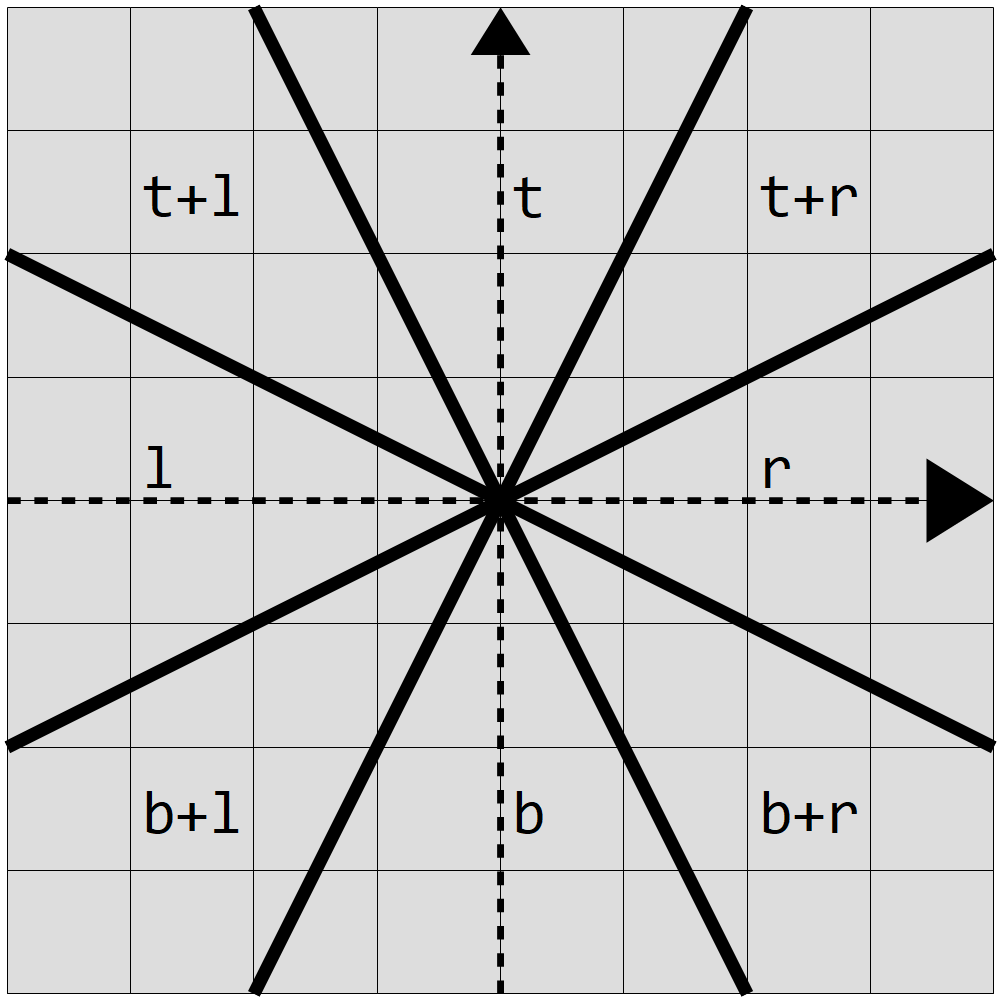
\includegraphics[height=3cm]{relation_cone.png}
  \caption{Potential positions of an object to be only \textbf{t}op
    of, \textbf{r}ight of, \textbf{b}ottom of, or \textbf{l}eft of a
    reference object located in the origin. Also the four
    overlapping regions are indicated.}
  \label{fig:relations}
\end{figure}

%%% Based on the position proposals
%%% Show cone of relations
%%% (Also incorporate other relations than spatial?)

\subsubsection{Inferring Global Symbolic Explanations}

After the inference of visual parts and the relationships that hold
between them, we can build the BK needed for Aleph. Part affiliation
to an example can be declared by the \ilprule{contains} predicate. We
give all parts a unique name over all examples. Suppose part
\ilprule{A} is part of a particular example \ilprule{E} and describes
the human understandable concept $\text{\ilprule{c}} \in C$. Then the
example affiliation can be stated by the predicates
\ilprule{contains(E, A)}, \ilprule{isa(A, c)}.
Likewise for the relations we can use 2-ary predicates that state the
constellation that holds between the parts. When part \ilprule{A} is
left of part \ilprule{B} we incorporate the predicate
\ilprule{left\_of(A, B)} in the BK and likewise for the other
relations. When the BK for the positive and negative examples $E^+$
and $E^-$ is found, we can use Aleph's induction mechanism to find the
set of rules that best fit the examples. The complete algorithm for
the process is stated in Algorithm~\ref{alg:ex_gen}.

\begin{comment}
  Since we want to allow a certain degree of tolerance, we set the
  \emph{noise} hyperparameter $n$ of Aleph to a value above
  zero. This value gives the percentage of the maximally allowed
  false positives for an induced theory given the examples. That
  means, that a higher value allows for more negative examples to be
  covered by the rules, thus resulting in more general rules.
\end{comment}
%%% Write BK (also show how the predicates look like in Prolog syntax)

\begin{algorithm}[t]
  \caption{\label{alg:ex_gen} Verbal Explanation Generation for DNNs}
  \begin{algorithmic}[1]
    % \footnotesize
    \State \textbf{Require:} Positive and negative binary masks $M^+$, $M^-$
    \State \textbf{Require:} Pool of human understandable concepts $C$
    
    \State $E^+ \gets \{\}$
    \State $E^- \gets \{\}$
    \State \textbf{for each} $\odot \in \{+, -\}$ \textbf{do}
    \State ~~~\textbf{for each} $m^\odot \in M^\odot$ \textbf{do}
    \State ~~~~~~$P \gets \{\}$
    \State ~~~~~~\textbf{for each} $l_c \in m^\odot$ where $c \in C$ \textbf{do}
    \State ~~~~~~~~~$p_c \gets calculatePartPosition(l_c)$
    \State ~~~~~~~~~$P \gets P \cup \{\langle c, p_c \rangle\}$
    \State ~~~~~~$R \gets calculateRelations(P)$
    \State ~~~~~~$E^\odot \gets E^\odot \cup {\langle P, R \rangle}$
    \State $T \leftarrow$ Aleph$(E^+, E^-)$
    \State \textbf{return} $T$
  \end{algorithmic}
\end{algorithm}


%%% Local Variables:
%%% mode: latex
%%% TeX-master: "concept_embeddings_and_ilp"
%%% End:
